% LaTeX figure environment for the seed-42 cross-architecture fall-recall-vs-epsilon plot.
% Image: results/cross_architecture/figures/cross_architecture_seed42_fall_recall_vs_epsilon.png
% Source data commits: LeNet (3200a89), ResNet18 (3578136), GRU (40bd655),
%                      BiLSTM (c298471), Transformer/ViT (5202608).
% Requires \usepackage{graphicx}.

\begin{figure}[t]
  \centering
  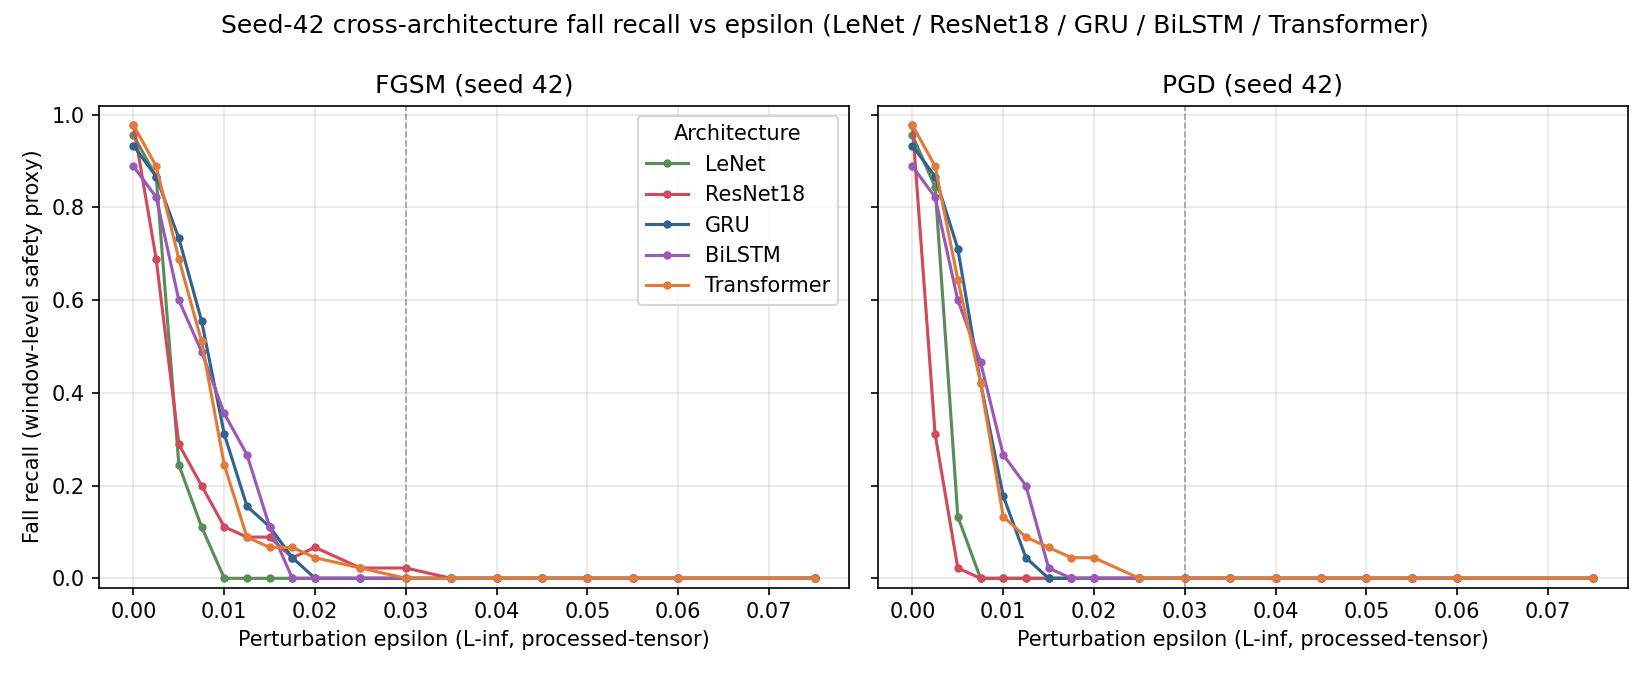
\includegraphics[width=\linewidth]{results/cross_architecture/figures/cross_architecture_seed42_fall_recall_vs_epsilon.png}
  \caption[Seed-42 cross-architecture fall recall vs.\ perturbation budget]{%
    Seed-42 cross-architecture pilot: window-level fall recall versus $L_\infty$
    perturbation budget $\varepsilon$ for five UT-HAR/SenseFi architectures
    (LeNet, ResNet18, GRU, BiLSTM, Transformer/ViT), shown as separate FGSM (left)
    and PGD (right) panels. Curves are single-seed (seed~42) on the held-out test
    split ($n=500$ windows, $45$ fall windows); the dashed vertical line marks the
    matched evaluation point $\varepsilon=0.03$. Perturbations are digital-domain,
    processed-tensor perturbations, not physical-layer or over-the-air attacks.
    All five architectures lose essentially all fall recall under PGD by
    $\varepsilon\le0.025$, and reach $0.000$ fall recall under PGD at
    $\varepsilon=0.03$. BiLSTM and the Transformer are included as
    temporal/attention-based robustness baselines (not fall-risk prediction).
    Priority~1 established five-seed reliability for the LeNet baseline; this
    figure is a single-seed cross-architecture pilot and is not a multi-seed
    cross-architecture result.}
  \label{fig:cross-arch-seed42-fall-recall}
\end{figure}
